\documentclass[10pt,portrait]{article}
\usepackage{amssymb,amsmath,amsthm,amsfonts}
\usepackage{multicol,multirow}
\usepackage{calc}
\usepackage{ifthen}
% \usepackage[a4paper, total={6in, 8in}]{geometry}
\usepackage[a4paper, portrait, margin=0.4in]{geometry}
\usepackage[colorlinks=true,citecolor=blue,linkcolor=blue]{hyperref}
\usepackage{graphicx}
\usepackage{cases}

\makeatletter
\renewcommand{\section}{\@startsection{section}{1}{0mm}%
                                {-1ex plus -.5ex minus -.2ex}%
                                {0.5ex plus .2ex}%x
                                {\normalfont\large\bfseries}}
\renewcommand{\subsection}{\@startsection{subsection}{2}{0mm}%
                                {-1explus -.5ex minus -.2ex}%
                                {0.5ex plus .2ex}%
                                {\normalfont\normalsize\bfseries}}
\renewcommand{\subsubsection}{\@startsection{subsubsection}{3}{0mm}%
                                {-1ex plus -.5ex minus -.2ex}%
                                {1ex plus .2ex}%
                                {\normalfont\small\bfseries}}
\makeatother
\setcounter{secnumdepth}{0}





\graphicspath{ {./images/} }







\begin{document}


\newpage
    \begin{center}
         \Large{\textbf{Event that will impact the market}} \\
    \end{center}


    \subsection{Tech company}
    \begin{itemize}
        \item CTO assign \& resign
        \item Policy change
        \item Investigation: privacy issue
        \item 
        \item 
        \item 
        \item 
    \end{itemize}


\newpage
    \begin{center}
         \Large{\textbf{The Story of Investment Horizon}} \\
         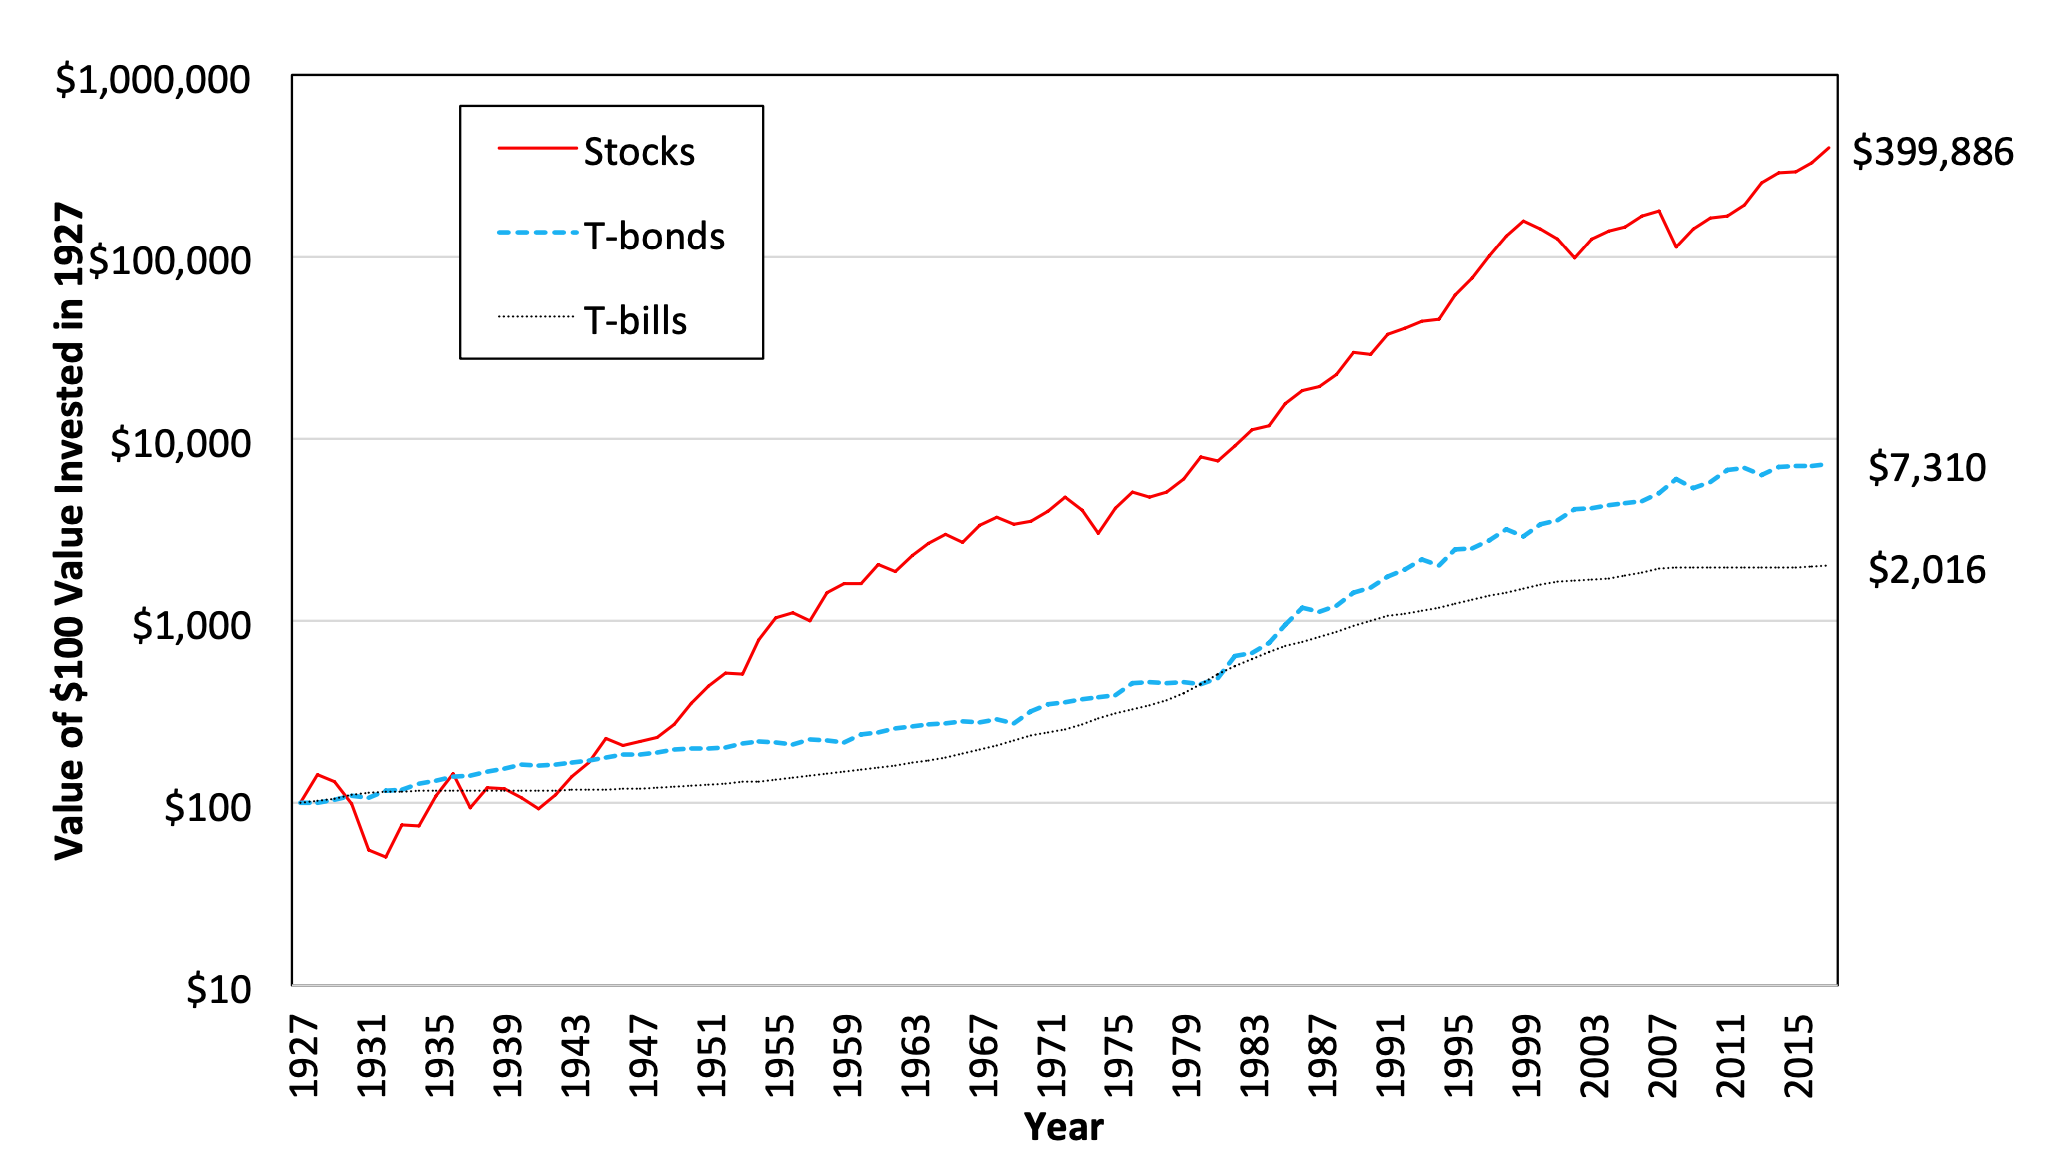
\includegraphics[width=0.8\textwidth]{asset_return_comparison}
    \end{center}

    \subsection{Stock is a good investment if you have long investment horizon}
    \begin{itemize}
        \item As we can tell from the graph, stock have significatlly greater return compared to bonds and bills.
        \item But bear in mind that this is true when you have a long investment horizon
        \item Put stock martket at a micro-scope level, we will experience great fluctuation everyday
    \end{itemize}
    
    \subsection{You can do better than stock, as long as you can take that risk}
    \begin{itemize}
        \item For instance, derivatives, are also a high risk asset, but the potential return is higher
        \item During the 2008 Crisis, there is a man who lend Goldman Sachs millions of money to help the firm.
        \item In exchange he asked for options on the stock with a low strike price
        \item Eventually Goldman Sachs survived the crisis and the man gain billions of money
        \item However, if we look at stock price, firms like Deutsche Bank never get out of the trouble. This trade is risky.
    \end{itemize}

    \subsection{Implication from my point of view}
    \begin{itemize}
        \item Take a long-term investment horizon and invest in things with high potential value
        \item We need to identify firms that is with good condition that worth invest in, E.g: Goldman Sachs v.s. Deutshce Bank
        \item This require us to know the business, how much company is involved in, the probability of it strive again.
    \end{itemize}

    \begin{center}
        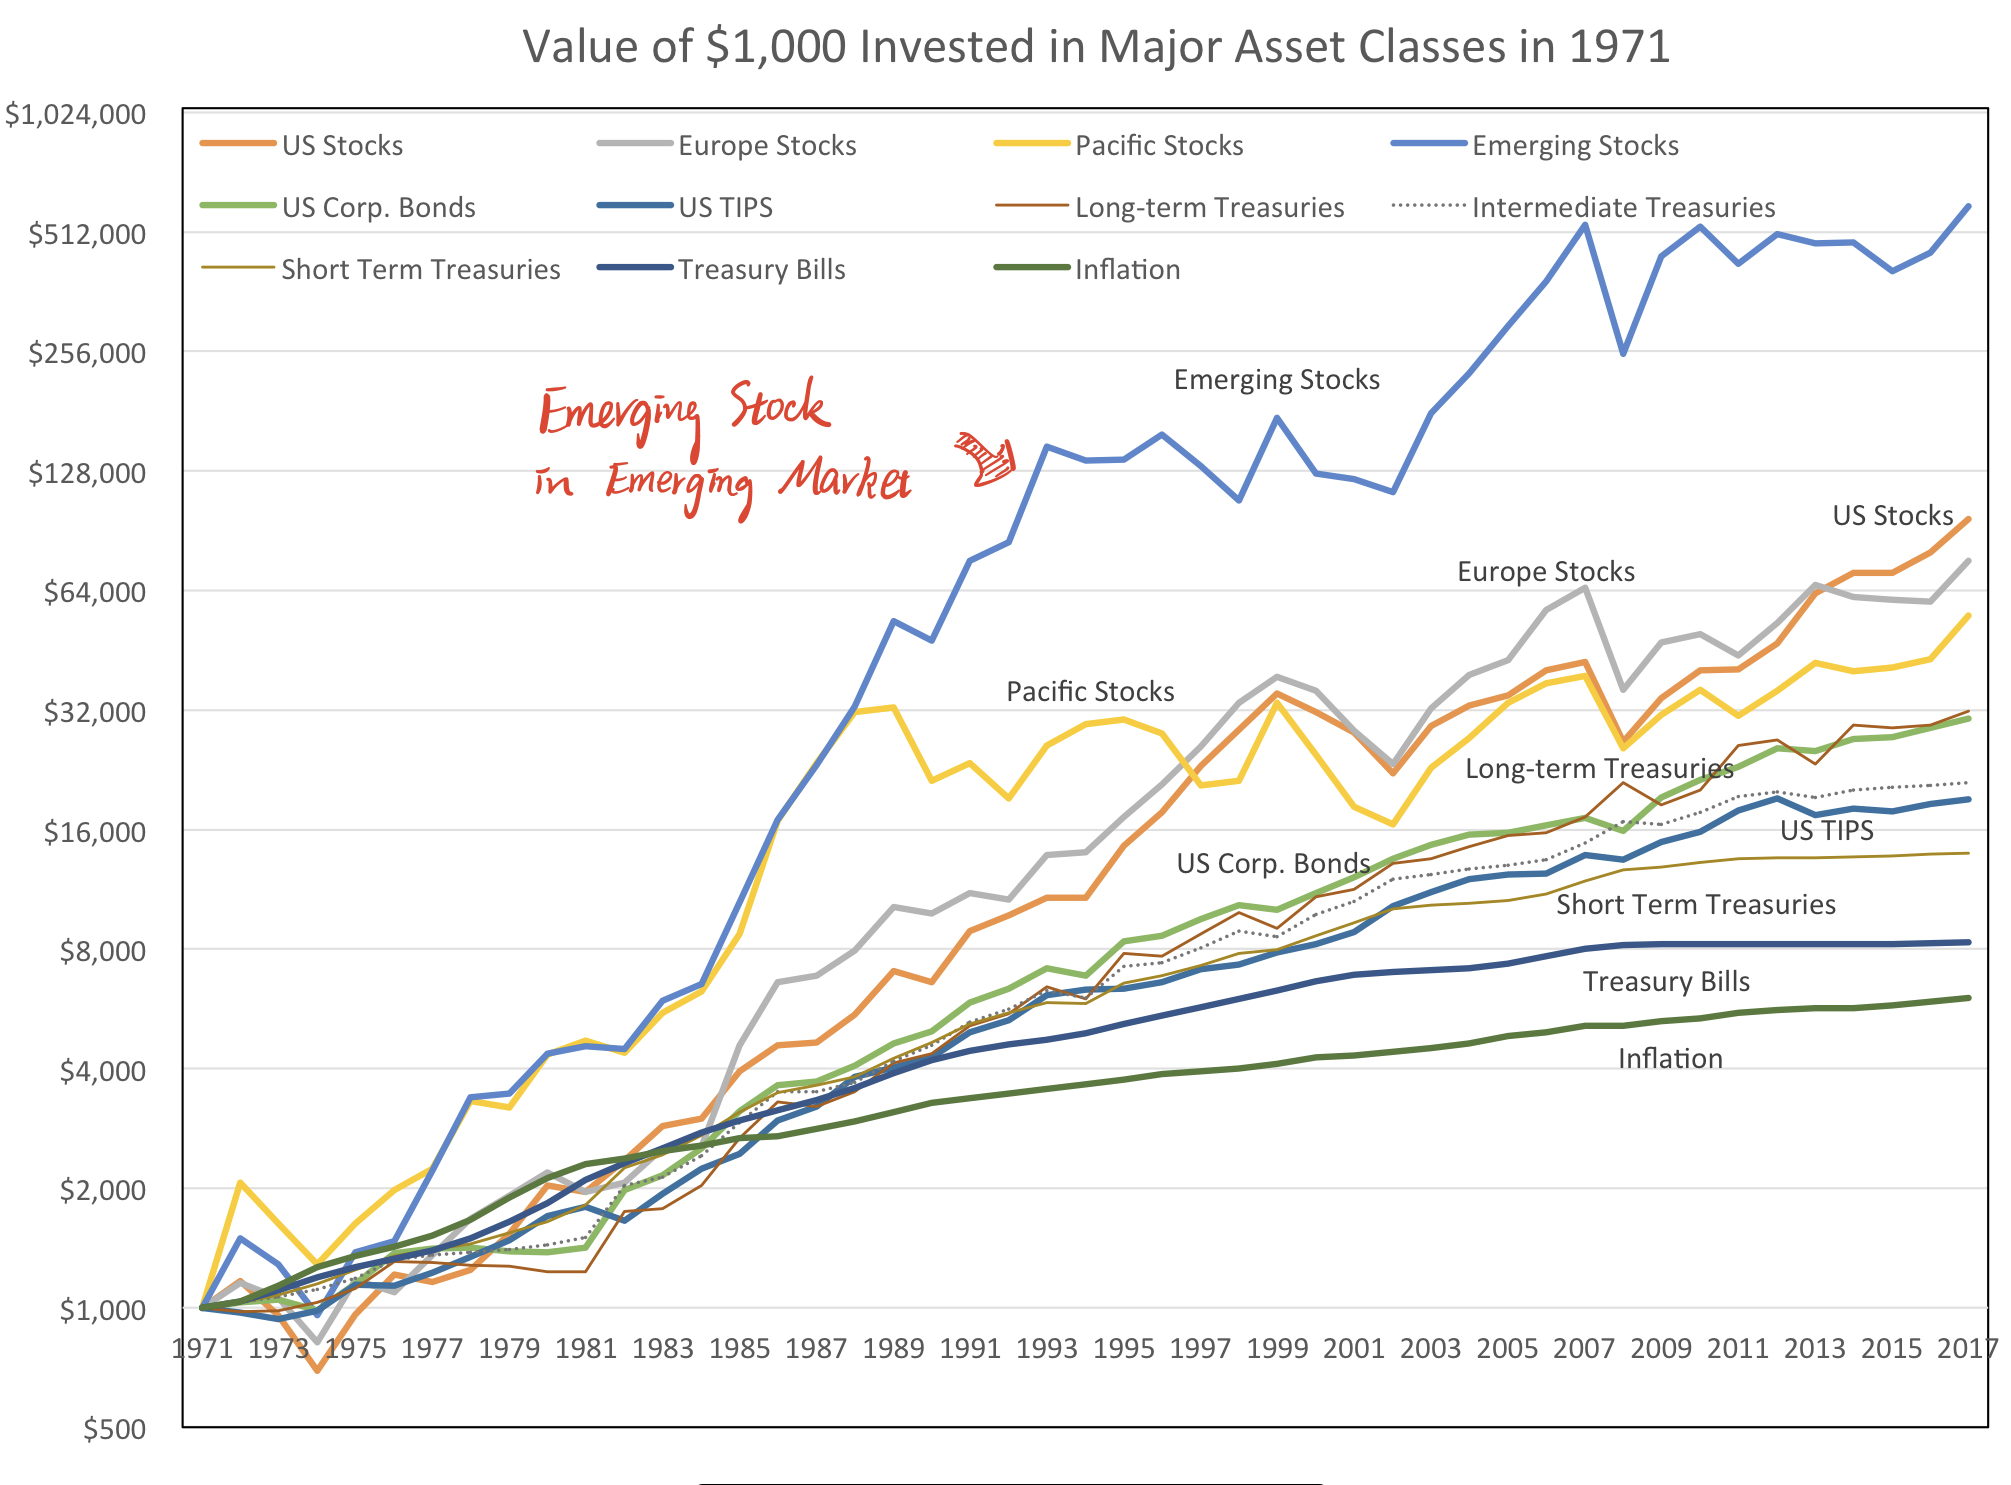
\includegraphics[width=0.6\textwidth]{asset_return_comparison_2}
    \end{center}


\newpage
    \begin{center}
         \Large{\textbf{Why investment with machine learning is so hard}} \\
         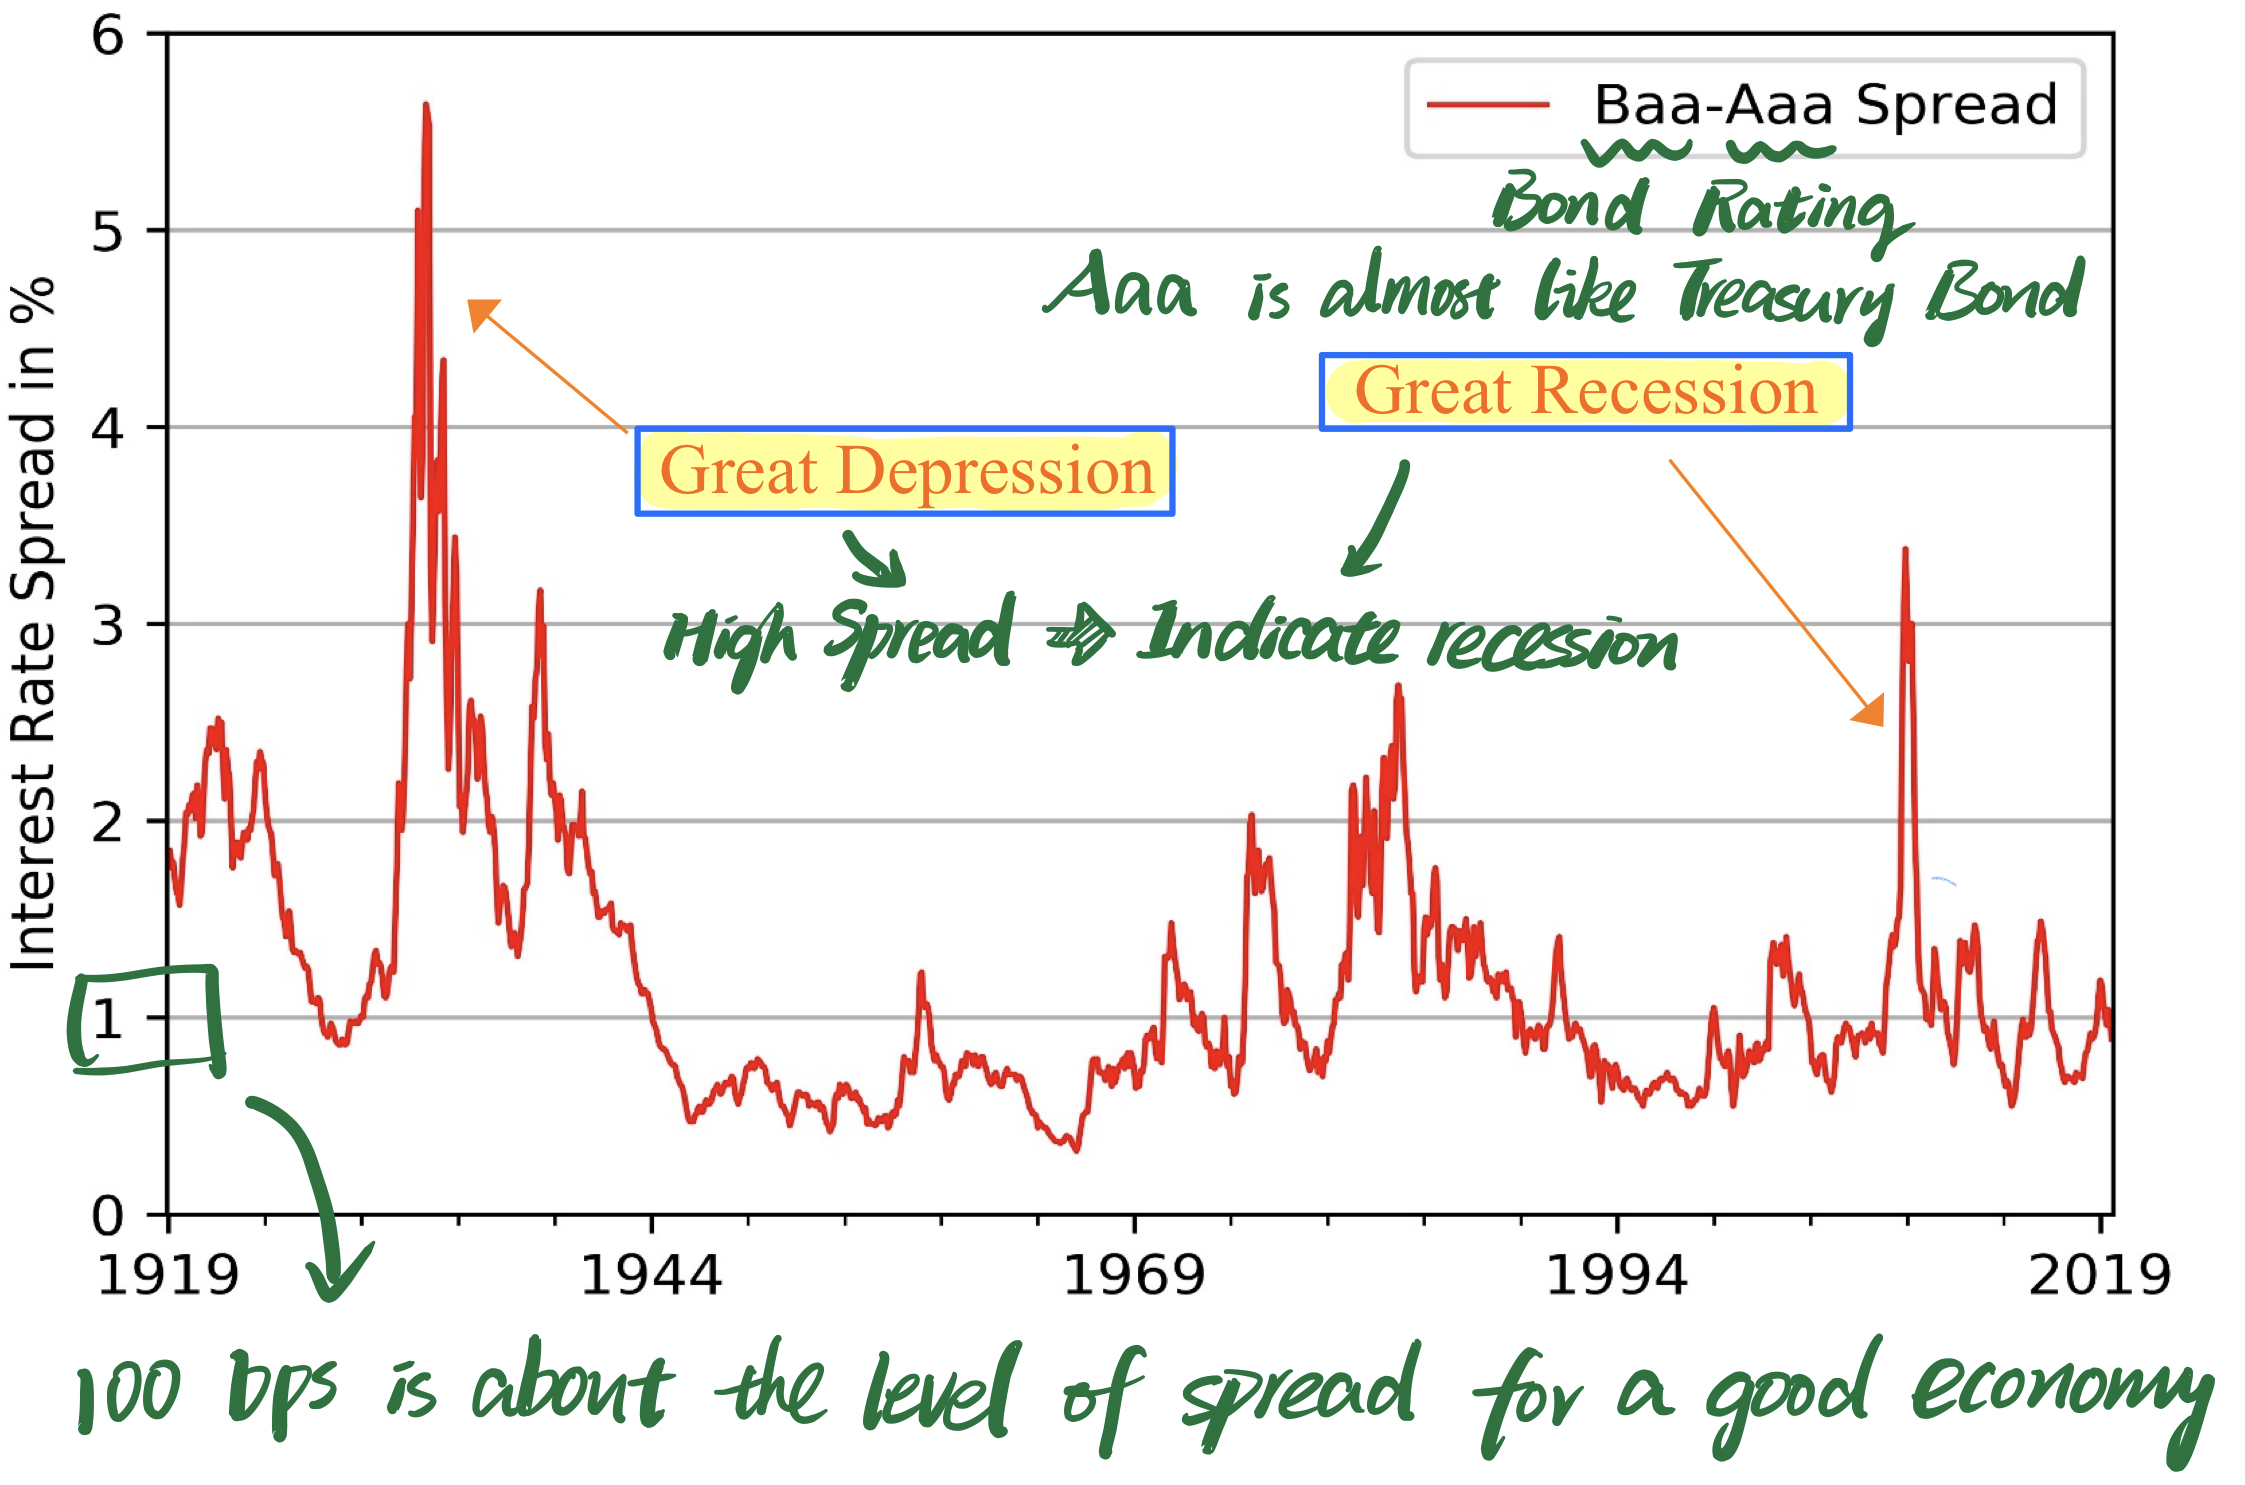
\includegraphics[width=0.9\textwidth]{interest-rate-spread}
    \end{center}


    \subsection{Interest rate spread is a good indicator for economic recession}
    \begin{itemize}
        \item The higher the spread, meaning that people is asking for a higher payoff for the risk
        \item usually a good and healthy economic keeps a spread aroud 100 basis points
    \end{itemize}

    \subsection{Interest rate spread as a good tool for adjusting economic behavior}
    \begin{itemize}
        \item If the spread is low, the investor will have no choice but to go for high risk investment
        \item By controlling the spread, we can stimulate the economy or make the economic slow down
    \end{itemize}

    \subsection{Interest rate spread as a good tool for adjusting economic behavior}
    \begin{itemize}
        \item If the spread is low, the investor will have no choice but to go for high risk investment
        \item By controlling the spread, we can stimulate the economy or make the economic slow down
    \end{itemize}

    \subsection{Implication}
    \begin{itemize}
        \item 
    \end{itemize}


\newpage
    \begin{center}
         \Large{\textbf{US Market in the recent years, related to DDM}} \\
    \end{center}


    \subsection{The corona virus makes the market to drop}
    \begin{itemize}
        \item it essentially drop the g, some guess is 0\%, some guess is 4\%
        \item some will say that the market has been crazy and the corona virus just bring it down
        \item before the crisis, the P/E is about 22, usually it is 17
        \item 
        \item 
    \end{itemize}

    \subsection{The central banks / fed make adjustment to lower interest rate}
    \begin{itemize}
        \item it essentially drop the k, from the CAPM model
        \item central bank wants to show support for the stock market
        \item 
        \item 
    \end{itemize}

    \subsection{When the stock market goes in crazy, people's risk averstion goes up the ceiling}
    \begin{itemize}
        \item $U_p = E(r_p) - \frac{1}{2}A\sigma_p^2$
        \item people goes in the 10 year treasury yields
        \item 
        \item 
    \end{itemize}

    \subsection{How to invest in light of different interest rate scenario}
    \begin{itemize}
        \item If the rate is low: we need to take advantage of this low borrowing cost and invest in more risky thing
        \item If the rate is high: borrowing money cost is high in the market, we adjust our position for less risky
    \end{itemize}

    \subsection{When talking return, we need to consider risk}
    \begin{itemize}
        \item What we need to focus on, is the sharp ratio
        \item It makes no sense just bring up the return, becuase a portfolio that is 2 times return the market can also be 2 times or even more volatile than the market
    \end{itemize}

    \subsection{How would presidential election influence the market}
    \begin{itemize}
        \item If bernie sander get nominated and compete with Donald Trump, the market will swing a lot since they are representing 2 different sides of government policy. Sander means more regulation and Trump stands for a less regulated and thus more free market. In this case, market volatility rise more, market risk premium rise more.
        \item If Joe Biden got nominated, the market will swing less since Biden is a mild / libral democrate, share more similarity with Trump in terms of the policy on market. In this case, market volatility rise less, market risk premium rise less.
    \end{itemize}

            % $
            % \begin{cases}
            %     \text{}\\
            %     \text{}\\
            %     \text{}\\
            %     \text{}\\
            % \end{cases}
            % $

            % \includegraphics[width=0.8\textwidth]{}


\newpage
    \begin{center}
         \Large{\textbf{Prudential}} \\
    \end{center}


    \subsection{Convexity}
    \begin{itemize}
        \item Larger convexity for liability?
        \item IG ? Investment grade ? where does this grade comes from?
        \item In stressful time, private asset tends to perform better?
    \end{itemize}


            % $
            % \begin{cases}
            %     \text{}\\
            %     \text{}\\
            %     \text{}\\
            %     \text{}\\
            % \end{cases}
            % $

            % \includegraphics[width=0.8\textwidth]{}


\newpage
    \begin{center}
         \Large{\textbf{The CAPM Anomalies}} \\
    \end{center}


    \subsection{}
    \begin{itemize}
        \item Russel index: index of smaller size, it is more volatile than SP500
        \item Lexi: online shopping
        \item Low B/M: market studied the company pretty well and the company is showing good perspective. While high book to market ratio may have the situation: it don't have sexy figure, but is indeed good.
        \item Betting against beta
        \item 
        \item 
        \item 
    \end{itemize}




% \newpage
%     \begin{center}
%          \Large{\textbf{Why investment with machine learning is so hard}} \\
%     \end{center}


    % \subsection{}
    % \begin{itemize}
    %     \item 
        % \item 
        % \item 
        % \item 
        % \item 
        % \item 
        % \item 
    % \end{itemize}


            % $
            % \begin{cases}
            %     \text{}\\
            %     \text{}\\
            %     \text{}\\
            %     \text{}\\
            % \end{cases}
            % $

            % \includegraphics[width=0.8\textwidth]{}

\end{document}